\documentclass[border=3pt]{standalone}
% Preâmbulo compartilhado pelos diagramas TikZ da aula 14 (SLAM com EIF)
\usepackage[T1]{fontenc}
\usepackage[utf8]{inputenc}
\usepackage{lmodern}
\usepackage{amsmath}
\usepackage{xcolor}
\usepackage{tikz}
\usetikzlibrary{arrows.meta,angles,quotes,decorations.pathmorphing,decorations.pathreplacing,calc,
                positioning,shapes.geometric,shapes.misc,backgrounds,fit,
                math}

% Paleta (mesma dos SVGs originais)
\definecolor{dblue}{HTML}{2A5B8C}
\definecolor{dorange}{HTML}{B3541E}
\definecolor{dgreen}{HTML}{4A7C59}
\definecolor{dred}{HTML}{9C4B4B}
\definecolor{dcream}{HTML}{F4F1EA}
\definecolor{dshade}{HTML}{DDD7C9}

% Função gaussiana (não normalizada por padrão de escala visual)
\pgfmathdeclarefunction{gauss}{3}{%
  \pgfmathparse{1/(#3*sqrt(2*pi))*exp(-((#1-#2)^2)/(2*#3^2))}%
}

% Estilos comuns (prefixo d... para não colidir com chaves internas do pgf)
\tikzset{
  >={Stealth[length=2mm]},
  dguide/.style={gray!55, dashed, line width=0.4pt},
  daxis/.style={gray!60, line width=0.7pt, ->},
  dbody/.style={fill=black!3, draw=black!80, line width=1pt},
  dacc/.style={draw=dblue, line width=1pt},
  dlbl/.style={black!55, font=\small},
  dsub/.style={black!45, font=\footnotesize},
  dstate/.style={circle, draw=black!80, fill=dcream, line width=1pt,
                 minimum size=17mm, font=\large, inner sep=1pt},
  dobs/.style={circle, draw=black!80, fill=dshade, line width=1pt,
               minimum size=14mm, font=\large, inner sep=1pt},
  dbox/.style={rounded corners=2pt, draw=black!80, fill=dcream, line width=1pt,
               align=center, inner sep=6pt},
  dop/.style={circle, draw=black!80, fill=white, line width=1pt,
              minimum size=6mm, inner sep=0pt, font=\small},
  dtrans/.style={->, dblue, line width=1pt},
  dmeas/.style={->, dorange, line width=1pt},
  dcurve/.style={line width=1pt, dblue},
  dcurveb/.style={line width=1.4pt, dorange},
}

\begin{document}
\hyphenpenalty=10000 \exhyphenpenalty=10000 \tolerance=9999 \emergencystretch=3em
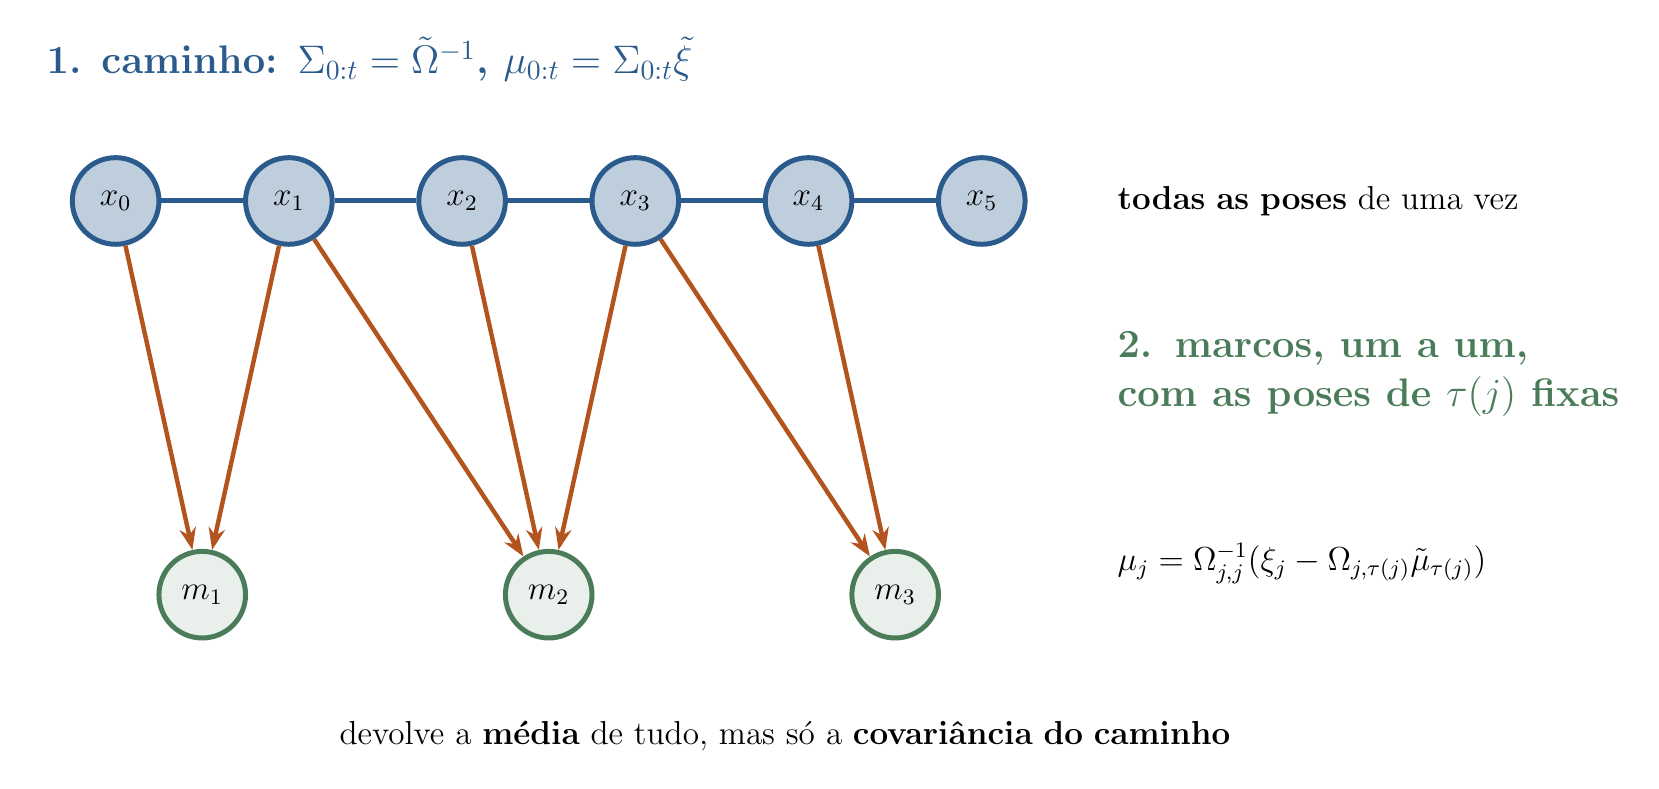
\begin{tikzpicture}[x=1cm,y=1cm]
\tikzset{p/.style={circle, draw=dblue, fill=dblue!30, line width=1.8pt, minimum size=1.1cm, font=\large},
        m/.style={circle, draw=dgreen, fill=dgreen!12, line width=1.8pt, minimum size=1.1cm, font=\large}}
\node[font=\Large\bfseries, text=dblue, anchor=west] at (0.0,8.4) {1. caminho: $\Sigma_{0:t}=\tilde\Omega^{-1}$, $\mu_{0:t}=\Sigma_{0:t}\tilde\xi$};
\foreach \i in {0,...,5} {\node[p] (x\i) at ({1.0+\i*2.2},6.6) {$x_\i$};}
\foreach \i/\j in {0/1,1/2,2/3,3/4,4/5} {\draw[dblue, line width=1.8pt] (x\i) -- (x\j);}
\node[font=\large, anchor=west, text width=6.4cm] at (13.6,6.6) {\textbf{todas as poses} de uma vez};
\node[font=\Large\bfseries, text=dgreen, anchor=west, text width=6.4cm] at (13.6,4.4) {2. marcos, \textbf{um a um}, com as poses de $\tau(j)$ \textbf{fixas}};
\node[m] (m1) at (2.1,1.6) {$m_1$}; \node[m] (m2) at (6.5,1.6) {$m_2$}; \node[m] (m3) at (10.9,1.6) {$m_3$};
\foreach \p/\q in {x0/m1,x1/m1,x1/m2,x2/m2,x3/m2,x3/m3,x4/m3} {\draw[->, dorange, line width=1.6pt, -{Stealth[length=2.8mm]}] (\p) -- (\q);}
\node[font=\large, anchor=west, text width=6.4cm] at (13.6,2.0) {$\mu_j=\Omega_{j,j}^{-1}(\xi_j-\Omega_{j,\tau(j)}\tilde\mu_{\tau(j)})$};
\node[font=\large, text width=19cm, align=center] at (9.5,-0.2) {devolve a \textbf{média} de tudo, mas só a \textbf{covariância do caminho}};
\end{tikzpicture}
\end{document}
